\Chapter{App.vue működése}

\Section{Vue.js bemutatása}

A Vue.js egy JavaScript keretrendszer, melynek fejlesztését Evan You kezdte el, és 2014-ben jelent meg először. Célja az volt, hogy egy könnyű keretrendszert készítsen az Angular előnyeinek megtartásával. A Vue.js egy MVC-hez hasonló architektúrát követ. Adataink, függvényeink, illetve a HTML megjelenítés remekül szétválasztható, ami miatt összességében egy átláthatóbb kódot kapunk eredményül. Egy Vue alkalmazás komponensekből épül fel, melyek akár többször is felhasználhatók ugyanazon alkalmazás részeként.

\begin{figure}[h!]
\centering
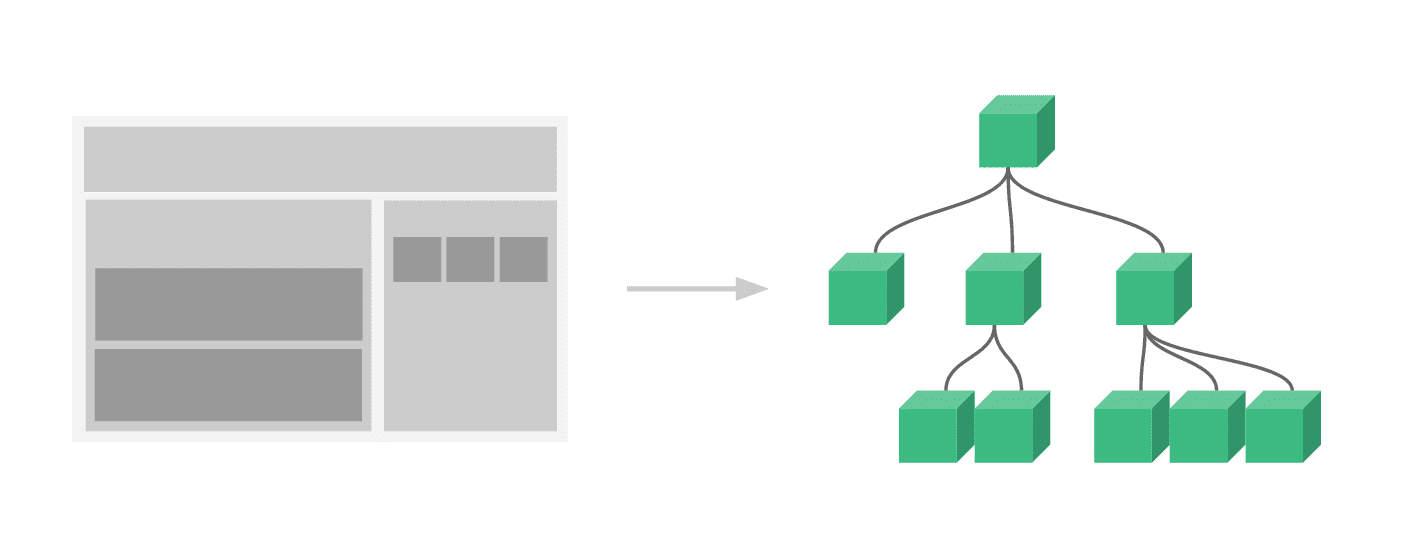
\includegraphics[scale=0.25]{images/components.png}
\caption{VueJS komponens kapcsolatok}
\label{fig:ff}
\end{figure}

A következő szakaszokban nézzük is meg egy Vue projekt megvalósítást, komponensekkel együtt, lépésenként.

\subsection{Projekt létrehozása}

Egy Vue projekt létrehozásához egyaránt használhatunk parancsoros vagy grafikus felülettel rendelkező \textit{wizard}-ot. A következő lépések a grafikus felülettel történő projekt létrehozást mutatják be.
\begin{enumerate}
  \item Nyitunk egy terminált, majd beírjuk a következő parancsot: vue ui
\begin{figure}[h!]
\centering
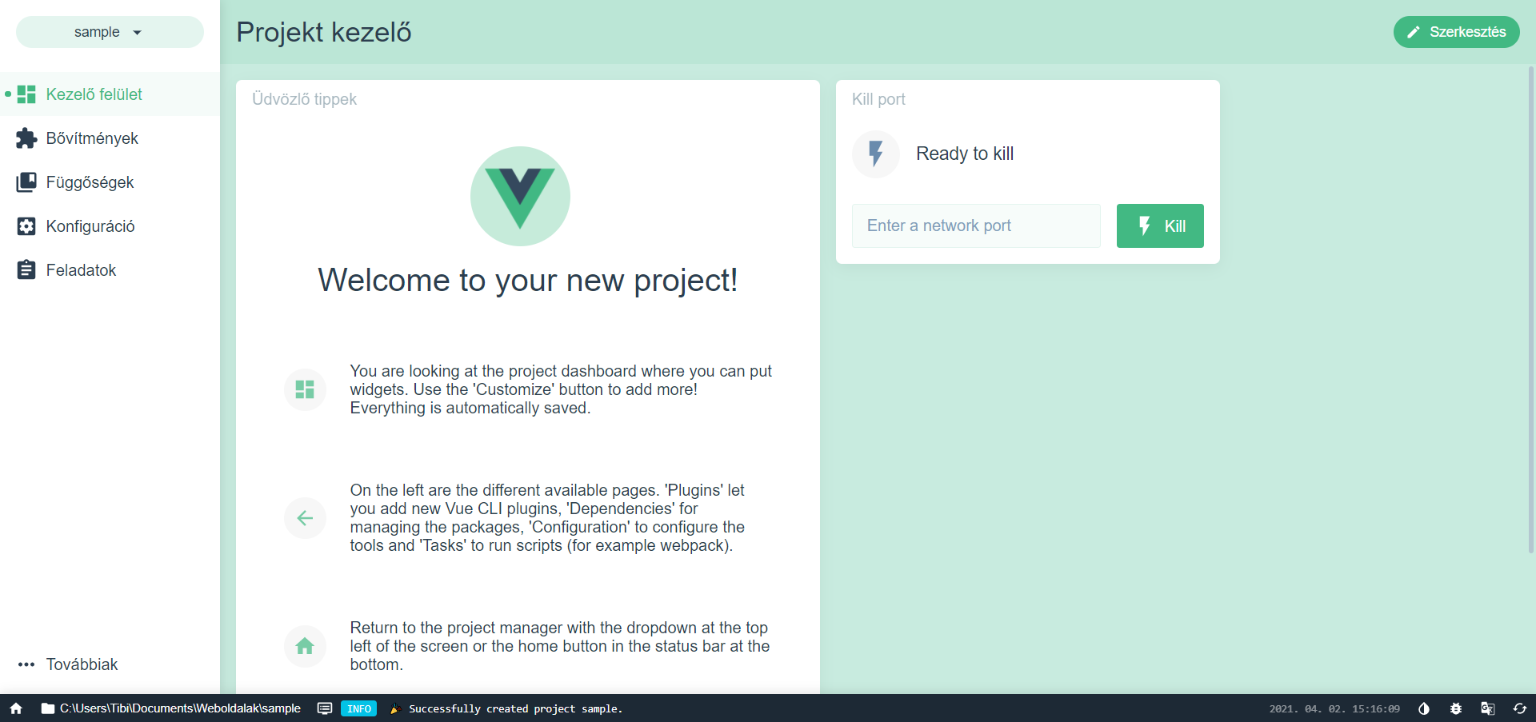
\includegraphics[width=\textwidth]{images/1617369552704.png}
\caption{VueJS projekt kezelő}
\label{fig:ff}
\end{figure}
A parancs beírását követően egy projekt kezelő nyílik meg a böngészőnkben.
\newpage
  \item Kattintsunk a “Továbbiak” gombra, majd a “Vue projekt kezelő”-re.
  \item Nyissuk meg a “Létrehozás” fület, majd válasszuk ki, hogy hova szeretnénk létrehozni az új vue projektünket.

  \item Nevezzük el a projektet, majd kattintsunk a “Következő” gombra.

  \item Válasszuk ki, hogy melyik Vue verziót szeretnénk alkalmazni. Én ebben a példában a Vue2-t fogom választani. Ha készen vagyunk, kattintsunk a “Create
  \item Nyitunk egy terminált, majd beírjuk a következő parancsot: vue ui
\begin{figure}[h!]
\centering
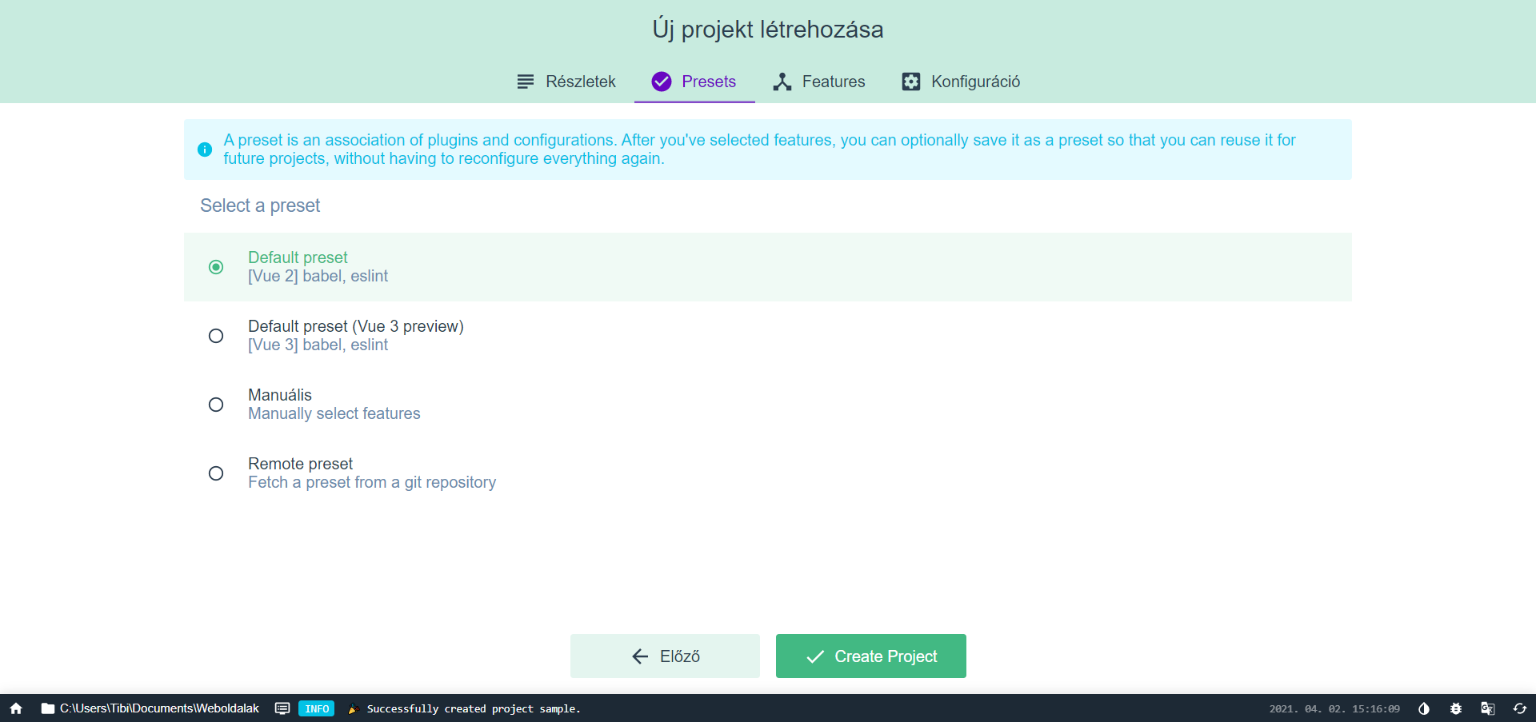
\includegraphics[width=\textwidth]{images/1617369965789.png}
\caption{Verzió kiválasztása}
\label{fig:ff}
\end{figure}
 \item A projektünk mappájában nyissunk meg egy terminált, majd írjuk be a következő parancsot: npm run serve
 \item Ha minden sikeres volt, nyissuk meg a böngészőbe a localhost:8080 URL-t.
	\begin{figure}[h!]
	\centering
	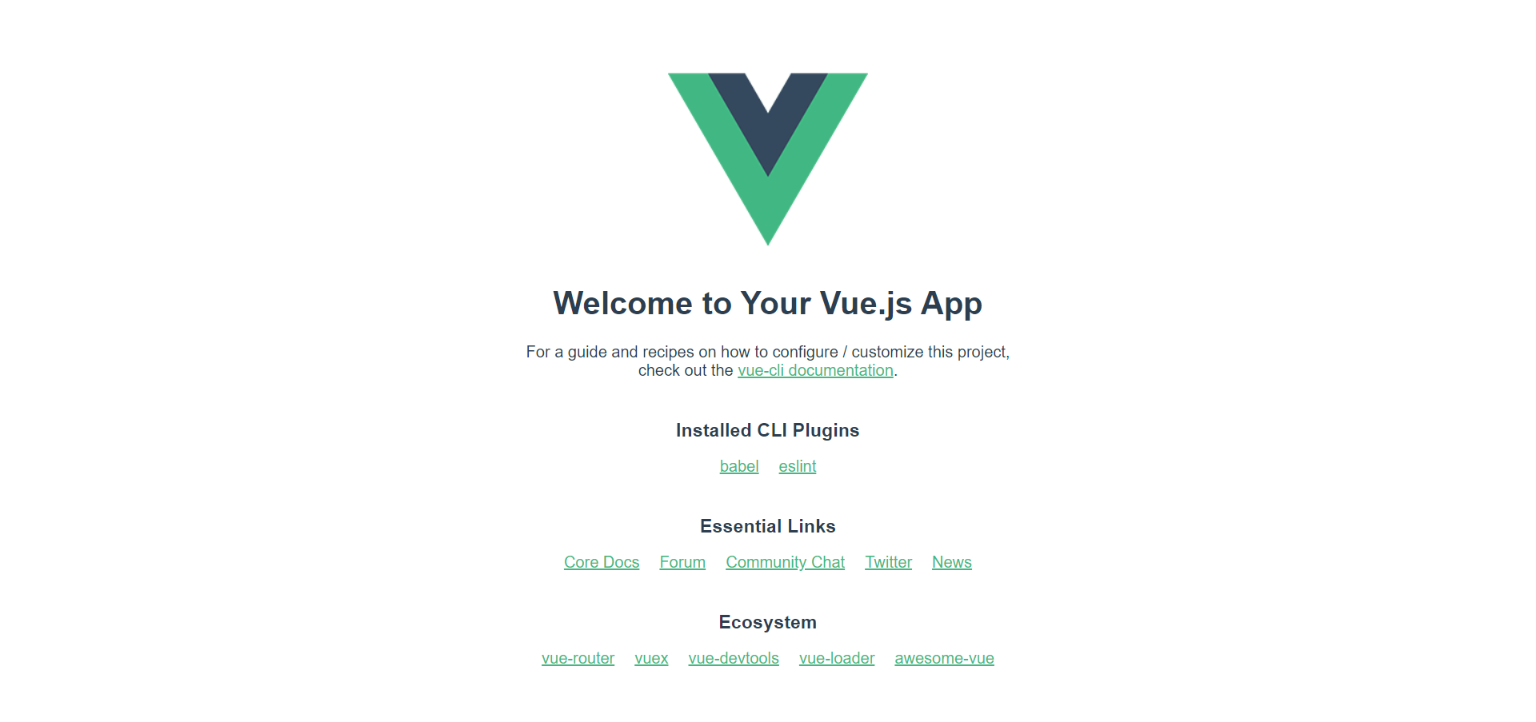
\includegraphics[width=\textwidth]{images/1617370382875.png}
	\caption{Kész projekt}
	\label{fig:ff}
	\end{figure}
\end{enumerate}

\subsection{Komponens hozzáadása}
\begin{enumerate}
	\item A projekt létrehozása során automatikusan generált nekünk a components mappán belül egy HelloWorld.vue nevű fájlt. Ebben a mappában érdemes tárolni más komponenseket is, a rendezettség és áttekinthetőség miatt. Ebből a fájlból kitörlöm azokat a részeket, amik a példába nem töltenek be szerepet. 
	\begin{figure}[h!]
	\centering
	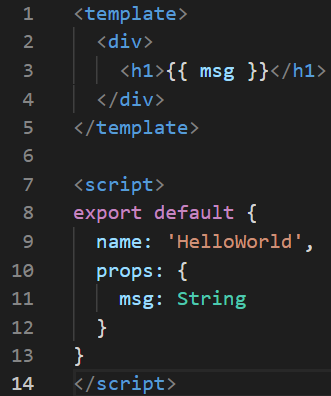
\includegraphics[scale=0.25]{images/14dfb7fd47c01c0cd6d8692ca740c349.png}
	\caption{Minta komponens kódja}
	\label{fig:ff}
	\end{figure}
	\begin{itemize}
		\item <template></template> tagek között a HTML megjelenés található.
		\item name - A komponens elnevezése.
		\item props - Ez egy tömb, melynek több adata is lehet, ezeket az értékeket várja az App.vue-tól.
	\end{itemize}
	\item Az App.vue-hoz, most hozzáadjuk a HelloWorld.vue komponenst. Ezt úgy tudjuk megtenni, hogy a <script></script> tagek között importáljuk a fájlt.
	\begin{javascript}
import HelloWorld from './components/HelloWorld.vue'
\end{javascript}
	Illetve a “components” tagjához is hozzáadjuk:
\begin{javascript}
components: {
  HelloWorld
}
	\end{javascript}

 \item Nincs más dolgunk, mint alkalmazni a <template></template> tagek között. Ahhoz, hogy bemutassam, hogy egy komponenst kétszer is lehet használni különböző adatokkal ugyanabban az alkalmazásban a következőként fogom alkalmazni:

\begin{verbatim}
<HelloWorld msg="Én vagyok az első komponens"/>
<HelloWorld msg="Ugyanolyan komponens vagyok, csak más értékkel"/>
\end{verbatim}
Íme az eredmény:
\begin{figure}[h!]
	\centering
	
\includegraphics[scale=0.25]{images/1617372108829.png}
	\caption{Példa megjelenítése}
	\label{fig:ff}
	\end{figure}
\end{enumerate}

\Section{Változók}
\begin{itemize}
	\item socket: {}, - Szerverhez való kapcsolódáshoz szükséges
	\item name:'Anonymus', - Játékos neve
	\item skin:null, - Játékos kinézete
	\item status:'connecting', - Játékos aktuális státusza
	\item ingame:false, - Játékban való részvétel
	\item isActive:false, - Éppen a játékos van-e soron az adott körben
	\item isBuying:false, - Megvásárolható ingatlanon áll-e a játékos
	\item isInventoryCheck:false, - Nézi-e valaki inventory-át a játékos
	\item isSellCheck:false, - Az Eladás menüpontban van-e a játékos
	\item isUpgradeCheck:false, - A Fejlesztés menüpontban van-e a játékos
	\item isDestroyCheck:false, - A Bontás menüpontban van-e a játékos
	\item isTradeCheck:false, - A Csere menüpontban van-e a játékos
	\item tradeStatus:0, - A játékos státusza az aktuális cserében
	\item isTrading:false, - A játékos éppen kereskedik-e
	\item tradeWindow:null, - A kereskedésben megadott információkat tárolja
	\item inventoryCheckName:'', - Játékos neve akinek az inventory-át éppen nézi
	\item skins:[], - Tárolja a beolvasott kinézeteket
	\item cards:[], - Tárolja a beolvasott kártyákat
	\item messages:[], - Tárolja a szervertől kapott üzeneteket
	\item jailtime:null, - Játékos aktuális börtönideje
	\item freecard:0, - Játékos aktuális ingyen szabadulhatsz a börtönből kártyái
	\item money:0, - Játékos aktuális pénze
	\item doubleDice:0, - Hányszor dobott a játékos mióta ő van körön (dupla illetve tripla dobások miatt szükséges)
	\item game:new Game() - Aktuális játék állása
\end{itemize}

\Section{Kommunikáció a szerverrel}
Abban az esetben, hogyha kérést szeretnénk indítani a szerver felé, a

\begin{verbatim}
this.socket.emit('sendmessageSocket',{msg:data,sender:this.name});
\end{verbatim}

függvényt kell alkalmaznunk. A 'sendmessageSocket' lesz a kérés, a 
\begin{javascript}
{msg:data,sender:this.name}
\end{javascript}
pedig az objektum, amit küldeni szeretnénk. Ez természetesen lehet egy egyszerű érték is. A szerver ezt a

\begin{verbatim}
socket.on('sendmessageSocket', (data) => {
  //…
}
\end{verbatim}

függvénnyel kezeli le. Fordített esetben, ha a szerver szeretne utasítást küldeni a kliensnek, ezt megteheti a

\begin{javascript}
io.emit('sendmessageFromSocket', (messages));
\end{javascript}

illetve

\begin{javascript}
socket.emit('sendmessageFromSocket', (messages));
\end{javascript}

függvényekkel is. A különbség közöttük, hogy az io.emit az összes szerveren lévő kliensnek kiküldi ezt az utasítást, a socket.emit viszont csak az éppen aktuális kliensnek, aki kérést intézett a szerver felé.

\subsection{Kérés küldése komponensből}
Esetemben több olyan alkalomra is sor került, amikor egy vue komponensből kellett kérést küldenem a szerver felé. Általában ezt úgy szokták megoldani egy vue alkalamzásban, hogy először az App.vue-ba emitelnek a következő módon:
\begin{javascript}
this.$emit('sendmsg',(this.cMsg));
\end{javascript}%$
Az App.vue-nak ezután ezt lekell kezelnie.
\begin{verbatim}
<Chat @sendmsg="getMessage(\$event)" … />
\end{verbatim}%$
Láthatjuk, hogy a Chat komponensből érkezett a kérés sendmsg néven. Ennek hatására lefut a getMessage funkció az App.vue-ban:
\begin{javascript}
getMessage(data){
  this.socket.emit('sendmessageSocket', {
    msg: data, sender: this.name
  });
}
\end{javascript}
Ez a függvény tovább küldi a szervernek egy kérést, illetve vele együtt a kapott adatokat.

\Section{Komponensek}

\begin{itemize}
	\item OnlinePlayers, - Játékosok adatainak megjelenítésére szolgáló felület.
	\item Login, - Bejelentkező felület.
	\item Waiting, - Várakozó felület.
	\item Table, - Játéktábla, emellett a használható gombok is ezen a komponensen belül található.
	\item Chat, - Kommunikációs felület.
	\item Inventory, - Az aktuálisan kiválasztott játékos megvásárolt bizniszeit/szolgáltatóit/telkeit jeleníti meg.
	\item Sell, - Értékek eladására szolgáló felület.
	\item Upgrade, - Telkek fejlesztésére szolgáló felület.
	\item Destroy, - Telkek bontására alkalmas felület.
	\item Trade, - Ebben a komponensben lehet kezdeményezni egy kereskedést.
	\item TradePartner - Hasonló a Trade komponenshez, viszont ez a másik fél szemszögében jelenik meg.
\end{itemize}